\documentclass{beamer}

\usetheme{Pittsburgh}
\useinnertheme{default}
\setbeamertemplate{footline}[page number]
\setbeamertemplate{navigation symbols}{}

\usepackage[utf8]{inputenc}
\usepackage{listings}
%\usepackage{proof}
\newcommand{\sub}{<:}
\newcommand{\infer}[2]{{#2 \over #1}}
\lstset{ %
language=Ruby,                % choose the language of the code
basicstyle=\footnotesize,       % the size of the fonts that are used for the code
numbers=left,                   % where to put the line-numbers
numberstyle=\footnotesize,      % the size of the fonts that are used for the line-numbers
stepnumber=0,                   % the step between two line-numbers. If it's 1 each line 
                                % will be numbered
numbersep=5pt,                  % how far the line-numbers are from the code
backgroundcolor=\color{white},  % choose the background color. You must add \usepackage{color}
showspaces=false,               % show spaces adding particular underscores
showstringspaces=false,         % underline spaces within strings
showtabs=false,                 % show tabs within strings adding particular underscores
frame=none,	                % adds a frame around the code
tabsize=2,	                % sets default tabsize to 2 spaces
captionpos=b,                   % sets the caption-position to bottom
breaklines=true,                % sets automatic line breaking
breakatwhitespace=false,        % sets if automatic breaks should only happen at whitespace
title=\lstname,                 % show the filename of files included with \lstinputlisting;
                                % also try caption instead of title
escapeinside={\%*}{*)},         % if you want to add a comment within your code
emph={add,output,input,icecast,single,playlist,file,
              fallback,crossfade,http,fade,initial,final,cross},            % if you want to add more keywords to the set
keywordstyle=\color[rgb]{0,0.5,0.3},
emphstyle=\color{red},
stringstyle=\color{blue},
}

\newcommand{\kw}[1]{{\color{red} #1}}

\usepackage{tikz}
\usepackage[all]{xy}

\renewcommand{\emph}[1]{\alert{#1}}
\renewcommand{\textbf}[1]{{\color{blue} #1}}

%\newtheorem{lemme}{Lemme}
%\newtheorem{theorem}{Theorem}
\newtheorem{proposition}{Proposition}
%\theoremstyle{definition}
%\newtheorem{definition}{Definition}

% \author{David Baelde for Savonet}
\title{\emph{\LARGE Liquidsoap} \\
  A High-Level Programming Language for \\ Multimedia Streaming}
\author{David Baelde\inst{1} \and Romain Beauxis\inst{2} \and Samuel Mimram\inst{3}}

\institute[Tulane University and others]
{
  \inst{1}%
  University of Minnesota, USA
  \and
  \vskip-2mm
  \inst{2}%
  Department of Mathematics, Tulane University, USA
  \and
  \vskip-2mm
  \inst{3}%
  CEA LIST -- LMeASI, France
}

\date[SOFSEM 2011]{SOFSEM 2011, Nový Smokovec -- Slovakia}

\begin{document}

\begin{frame}
  \maketitle
\end{frame}

\begin{frame}

\vfill

\begin{center}
{\LARGE
Simple things should be simple, \\[1ex]
Complex things should be possible.
}
\begin{flushright}
Alan Kay \hspace{0.5cm} ~
\end{flushright}
\end{center}

\vfill

\end{frame}

%% ===========================================

\begin{frame}[fragile]{Simple things}

\begin{lstlisting}
       output.icecast(%vorbis,
                      mount="radio.ogg",
                      single("music.mp3"))
\end{lstlisting}

\end{frame}

%% ===========================================

\begin{frame}{Complex things}

\begin{example}[Radio Pi]
\begin{itemize}
\item \emph{Several channels}: jazz, rock, techno, metal, etc.
\item Main channel relaying thematic ones depending on the time
\item \emph{Several outputs per channel}, various bitrates and formats
\item Interface with a web-based \emph{file scheduler}
\item \emph{Live shows} selectively relayed on various thematic channels
\item Volume normalization using \emph{Replay Gain}
\item Smart \emph{cross-fading} and various transitions
\item \emph{Blank detection} for live and files
\item etc.
\end{itemize}
All this in \emph{one instance} of liquidsoap.
\end{example}

\end{frame}

%% ===========================================

\begin{frame}{Background}

\begin{block}{The Savonet team}
Open-source development since \emph{2003}, unfunded
\begin{center}
David Baelde, Romain Beauxis and Samuel Mimram \\
Peter Brookes, Vincent Tabard\ldots
\end{center}
Languages: mostly \emph{OCaml}, also C and various script languages
\end{block}

\vfill

\begin{block}{Community}
\begin{itemize}
\item An established user base (bug reports)
\item Reaching the point where users help each other
\end{itemize}
\end{block}

\end{frame}

\begin{frame}{Recipe}

\begin{block}{Liquidsoap}
\begin{enumerate}
\item<1-> A script language
\item<2-> A notion of {\em source} (interactive stream generator)
\item<3-> Interfaces: libraries, external and remote applications
\end{enumerate}
\end{block}

\end{frame}

%% ===========================================

\begin{frame}[fragile]{Designing a stream}

\[
\xymatrix{
  *+[F]{\mathtt{input.http}}\ar[r]&*+[F]{\mathtt{fallback}}\ar[r]&
  *+[F]{\mathtt{normalize}}\ar[r]\ar[dr]&
  *+<10pt>[F=:<30pt>]{\mathtt{output.icecast}}\\
  *+[F]{\mathtt{playlist}}\ar[ur]& & & *+<10pt>[F=:<30pt>]{\mathtt{output.file}}\\
}
\]
\vfill
\pause

\begin{lstlisting}
live = input.http("http://server:8000/live.ogg")
music = playlist("/path/to/music")
s = fallback([live,music])
s = normalize(s)
output.icecast(%vorbis,mount="radio.ogg",s)
output.file(%mp3(bitrate=16),"/path/to/backup.mp3",s)
\end{lstlisting}

\end{frame}

%% ===========================================

\begin{frame}{Language design}

\begin{block}{Expressiveness vs.~Safety}
\begin{itemize}
\item<2-> Users should have maximum access to the model
\item<3-> The language should prevent mistakes, hide complexity
\end{itemize}
\end{block}

\onslide<4->
\begin{block}{Key techniques}
\begin{itemize}
\item<4-> Static types, inference
\item<5-> Functional language: immutability by default
\item<6-> Various analyses: fallibility, sharing\ldots
\end{itemize}
\end{block}

\end{frame}

%% ===========================================

\begin{frame}[fragile]{Transitions}

 \begin{center}
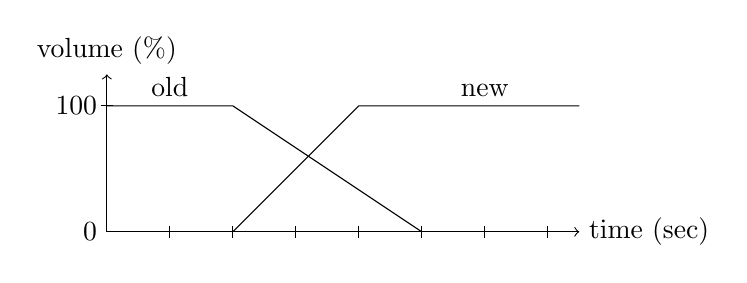
\begin{tikzpicture}[xscale=0.8,yscale=0.8]
\draw[->] (0,0) -- (0,2.5);
\draw (-0.1,2) -- (0.1,2);
\draw (0,2) node[anchor=east]{100};
\draw (0,0) node[anchor=east]{0};
\draw[->] (0,0) -- (7.5,0);
\foreach \x in {1,2,3,4,5,6,7} \draw (\x,-0.1) -- (\x,0.1);
\draw (0,2.5) node[anchor=south]{volume (\%)};
\draw (7.5,0) node[anchor=west]{time (sec)};
\draw (0,2) -- (2,2) -- (5,0);
\draw (2,0) -- (4,2) -- (7.5,2);
\draw (1,2) node[anchor=south]{old};
\draw (6,2) node[anchor=south]{new};
\end{tikzpicture}
\end{center}

\vfill
\pause
Complex thing:
\begin{lstlisting}
def mycross(old,new) =
  add([fade.initial(duration=2.,new),
       fade.final(duration=3.,old)])
end

# Apply mycross in between tracks
s = cross(duration=3.,mycross,s)
\end{lstlisting}
\end{frame}

\begin{frame}[fragile]{Transitions}

 \begin{center}
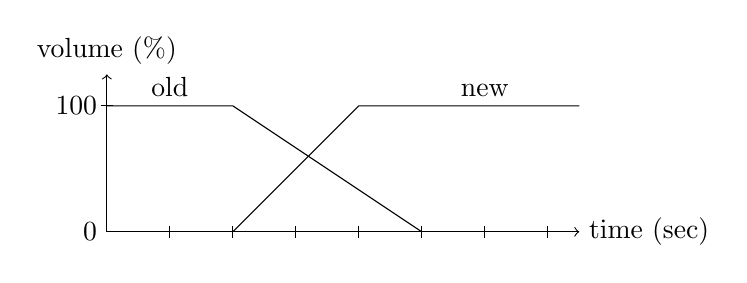
\begin{tikzpicture}[xscale=0.8,yscale=0.8]
\draw[->] (0,0) -- (0,2.5);
\draw (-0.1,2) -- (0.1,2);
\draw (0,2) node[anchor=east]{100};
\draw (0,0) node[anchor=east]{0};
\draw[->] (0,0) -- (7.5,0);
\foreach \x in {1,2,3,4,5,6,7} \draw (\x,-0.1) -- (\x,0.1);
\draw (0,2.5) node[anchor=south]{volume (\%)};
\draw (7.5,0) node[anchor=west]{time (sec)};
\draw (0,2) -- (2,2) -- (5,0);
\draw (2,0) -- (4,2) -- (7.5,2);
\draw (1,2) node[anchor=south]{old};
\draw (6,2) node[anchor=south]{new};
\end{tikzpicture}
\end{center}

\vfill
Simple things:
\begin{lstlisting}
s = crossfade(s)
\end{lstlisting}
\end{frame}

%% ===========================================

\begin{frame}{Features}

\begin{block}{Operators}
\begin{itemize}
\item Play a \kw{single} file, a \kw{playlist} or a queue of files
\item Play a file given by an external script
\item Switch, sequence, add
\item Sound processing: compression, change pitch, etc.
\item Event handlers: tracks, metadata, blank
\item \ldots
\end{itemize}
\end{block}

\begin{block}{Interfaces}
\begin{itemize}
\item Icecast, Shoutcast and compatible: output, relay and host
\item ALSA, OSS, Jack, Pulseaudio, AO\ldots
\end{itemize}
\end{block}

\textbf{Formats:} WAV, Ogg, MP3, AAC+, Flac, external

\textbf{Also}: requests and protocols, server, etc.

\end{frame}

\begin{frame}{Stream content}

\begin{center}
\large
  Each source has its own content type: \\
  any number of \textbf{audio video or midi} channels
\onslide<2->
\begin{flushright}
\small No cost for the user: content types are infered
\end{flushright}
\end{center}

\onslide<3->
\begin{block}{Traditional radio uses}
\begin{itemize}
\item Manual control over stereo/mono conversions
\item<4-> Produce many audio channels ({\em e.g.} dolby) for on-site playout, \\
  convert to stereo for web broadcast
\end{itemize}
\end{block}
\end{frame}

\begin{frame}[fragile]{Typing system for stream content}

Content type
\[
a\quad ::=\quad \star \;|\; 0 \;|\; S(a)
\]

\onslide<2->
Example:
\begin{center}
$(S(S(0)),S(\star),\star)$\\\medskip 
\onslide<3->
\begin{large}\texttt{source(2,*+1,*)}\end{large}
\end{center}

\onslide<4->
Type inference
   \[\infer{0\sub 0}{} \quad\quad
   \infer{S(A)\sub S(A')}{A\sub A'} \quad\quad
   \infer{\star\sub\star}{} \quad\quad
   \infer{0\sub \star}{} \quad\quad
   \infer{S(A)\sub \star}{A\sub\star}
\]
\[
   \infer{(A,B,C) \sub (A',B',C')}{A \sub A' \quad\quad B\sub B' \quad\quad C\sub C'}
\]

\end{frame}


\begin{frame}{Examples}
\begin{center}
   \texttt{
    \begin{tabular}{rcl}
    swap&:&(source(2,0,0)) -> source(2,0,0)\\
\onslide<2->
    on\_metadata&:&(handler,source('*a,'*b,'*c)) -> \\
    & & \hspace*{1cm}source('*a,'*b,'*c)\\
\onslide<3->
    echo&:&(delay:float,source('\#a,0,0)) -> \\
    & & \hspace*{1cm}source('\#a,0,0)\\
\onslide<4->
    greyscale&:&(source('*a,'*b+1,'*c)) -> \\
    & & \hspace*{1cm}source('*a,'*b+1,'*c)\\
\onslide<5->
    blank&:&() -> source('*a,'*b,'*c) \\
\onslide<6->
    output.file &:& 
       (format('*a,'*b,'*c),string,\\
     & & \phantom{(}source('*a,'*b,'*c)) -> \\
     & & \hspace*{1cm}source('*a,'*b,'*c)
    \end{tabular}
  }\end{center}
\end{frame}


\begin{frame}{Output content type}

Problem: Content type of outputs\\
\onslide<2->
Examples:
\begin{itemize}
 \item Sound card output
\begin{itemize}
\item<3-> Type: \texttt{(audio='\#a+1,video='\#b,midi='\#c)}\\
\item<4->\color{blue} Runtime verification
\end{itemize}
 \item<5-> Encoded output
\begin{itemize}
\item<6->\texttt{output.file(\%vorbis(channels=3),..)}
\item<7->\color{red} Type formats
\item<8->\texttt{\%vorbis(channels=3):format(3,0,0)}
\end{itemize}
\end{itemize}
\onslide<9->
\begin{center}
Trade-of: \color{green} Type inference vs. simplicity\end{center}



\end{frame}



%% ===========================================

\begin{frame}{Clocks}

\[
\xymatrix{
  \text{\only<3->{\color{red}}remote server A} \ar[dr] &
        & \mbox{\only<3->{\color{gray}}remote server B} \\
  \text{\only<3->{\color{blue}}soundcard 1} \ar[r]      &
                \text{liquidsoap} \ar[ur]\ar[r]\ar[dr]
        & \mbox{\only<3->{\color{blue}}soundcard 1}     \\
  \text{\only<3->{\color{green}}soundcard 2} \ar[ur] &
        & \mbox{\only<3->{\color{blue}}backup file}
}
\]

\vspace{0.5cm}
\pause

\begin{center}
\large
  A liquidsoap instance can control several clocks, \\
  each source assigned to a single clock
\onslide<5->
{\begin{flushright}
\small No cost for the user: clocks are infered
\end{flushright}}
\end{center}

\pause
\pause

%\begin{block}{Uses}
\onslide<4->
\begin{itemize}
\item Deal with drift and lags of external clocks
\item Avoid internal time inconsistencies (\kw{cross}, \kw{stretch}\ldots)
\end{itemize}
%\end{block}

\end{frame}

\begin{frame}[fragile]{Clocks}

\begin{lstlisting}
output.icecast(%vorbis,mount="myradio",
  fallback([crossfade(playlist("some.txt")),jingles]))
\end{lstlisting}

\onslide<2->
\scalebox{0.9}{
$\xymatrix{
   & *+[F]{\mathtt{playlist}}\ar[r]&*+[F]{\mathtt{crossfade}}\ar[r]&  *+[F]{\mathtt{fallback}}\ar[r]&
  *+[F]{\mathtt{output.icecast}}\\
   & &  & *+[F]{\mathtt{jingles}}\ar[u]& 
}$
}

\end{frame}

\begin{frame}[fragile]{Clocks}

\begin{lstlisting}
output.icecast(%vorbis,mount="myradio",
  fallback([crossfade(playlist("some.txt")),jingles]))
\end{lstlisting}

\scalebox{0.8}{
$\def\f{\save
*+<15pt>[F--]\frm{}\ar @{--} "2,2"\restore}%
\def\g{\save
"2,4"."1,2"."1,5"!C*+<27pt>[F--]\frm{}\ar @{--} "1,1"\restore}%
\xymatrix{
   {clock_1} & *+[F]{\mathtt{playlist}}\ar[r]\f&*+[F]{\mathtt{crossfade}}\ar[r]&  *+[F]{\mathtt{fallback}}\ar[r]&
  *+[F]{\mathtt{output.icecast}}\\
   &{clock_2} &  & *+[F]{\mathtt{jingles}}\ar[u]\g& 
}$
}

\end{frame}

\begin{frame}[fragile]{Clocks implementation}
 \begin{itemize}
  \item<2-> Not ruled by typing system
  \item<3-> Inferred at runtime
  \item<4-> Non-trivial cases: \texttt{add([s,crossfade(s)])}
  \item<5-> \textit{active} clocks vs. \textit{passive} clocks
  \item<6-> Available operators for power-users to sort out difficult cases
  \item<7-> Abstraction for multi-threading
 \end{itemize}

\end{frame}


%% ===========================================

\begin{frame}{Conclusion}

\begin{block}{Liquidsoap}
\begin{itemize}
\item<2-> A high-level language using theory of programming languages
\item<3-> A domain-specific language with non-programmer user-base
\item<4-> Many great features
\item<5-> A unique ability to combine them at will
\end{itemize}
\end{block}

\onslide<6->
\begin{block}{Future}
A deeper understanding of issues speficic
to continuous and discrete-events programming
\begin{itemize}
\item<7->More fine-grained language, notably for approaching DSP
\item<8->Relations with hybrid model simulators
\item<9->A new language combining our experience on Liquidsoap
with fundamental research
\end{itemize}
\end{block}

\vfill

\onslide<10->
\begin{center}
  \large \emph{Try liquidsoap!}
\end{center}

\end{frame}

\end{document}
